\scanpage{127}
% archive sheet number: 126
% source lines 1--4
\deleted{where the $\handwritten{\sigma}_i$ (resp. $\handwritten{\sigma}'_i$) are deduced from\deleted{s} $\handwritten{\sigma}$ (resp. from $\handwritten{\sigma}'$) by the three homomorphisms $\handwritten{\delta}_i:U\overset{\handwritten{\scriptscriptstyle\wedge}}{\unsure{\otimes|\Omega}}_kU\handwritten{\longrightarrow}U\overset{\handwritten{\scriptscriptstyle\wedge}}{\otimes}_kU\overset{\handwritten{\scriptscriptstyle\wedge}}{\otimes}_kU$ \deleted{using} $\handwritten{\Delta}\otimes\mathrm{id}_U$ and symmetric ones.} (NB I have not written out the calculation and do not guarantee the exact form of the hexagon relation).

% source lines 5--13
Let $k'$ be an algebra (commutative associative unital !) over $k$, whence $\unsure{\rlap{\(\mathrm u\)}U|\mathbb U}'=(U'_{\handwritten{\alpha}})$ and $\unsure{\rlap{\(\mathrm a\)}A|\mathbb A}'=\underset{\handwritten{\alpha}}{\underset{\handwritten{\longrightarrow}}{\lim}}A'_{\handwritten{\alpha}}$ over $k'$, with their structures o\rlap{'}f\deleted{algebra} bialgebras \handwritten{(}resp. bi-proalgebra for $U'$\handwritten{)}. We propose to determine the functors $G:C\handwritten{\to}\deleted{\mathrm{Modtf}(}\mathrm{Projf}(k')$\inserted{(projective modules of finite type over $k'$)\handwritten{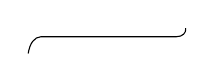
\begin{tikzpicture}[x=.4cm,y=.4cm,baseline=-.2ex]\draw (0,-.35) .. controls (.05,-.02) and (.2,.17) .. (.4,.18)--(4.7,.18) .. controls (4.90,.18) and (5.02,.3) .. (5.00,.45);\end{tikzpicture}}} \uline{exact and} $k$-\uline{linear}, equipped with an isomorphism $c:G(X\otimes Y)\handwritten{\simeq}G(X)\otimes G(Y)$. \deleted{\unsure{its}} First of all the datum of a right exact $G^{\deleted{k}}$\inserted{$C\handwritten{\to}\mathrm{Mod}(k')$}\handwritten{\begin{tikzpicture}[x=.4cm,y=.4cm,baseline=-.2ex]\draw (0,-.35) .. controls (.05,-.02) and (.2,.17) .. (.4,.18)--(2.5,.18) .. controls (2.70,.18) and (2.82,.3) .. (2.80,.45);\end{tikzpicture}} amounts to the datum of an $\rlap{(}L=(L_{\handwritten{\alpha}})$, \inserted{right\handwritten{\begin{tikzpicture}[x=.4cm,y=.4cm,baseline=-.2ex]\draw (0,-.35) .. controls (.05,-.02) and (.2,.17) .. (.4,.18)--(1.4,.18) .. controls (1.60,.18) and (1.72,.3) .. (1.70,.45);\end{tikzpicture}}} module over $U$\handwritten{,} equipped with a $k'$-module structure \deleted{over $k$} commuting with the operations of $U$ (NB $L_{\handwritten{\alpha}}=G(U_{\handwritten{\alpha}\unsure{s|S}})$ ), by
\[
G(\unsure{\rlap{\(X\)}M|\mathbb M})=L\otimes_U\rlap{\(X\)}M.
\]

% source lines 14--23
$k^{\deleted{\unsure{'}}}$-linearity means that the two structures over $k$ on $L$ coincide, i.e. that $L$ comes from a\deleted{e} module (pro) over $U'=(U'_{\handwritten{\alpha}})$ (each $L_{\handwritten{\alpha}}$ is a module over $U'_{\handwritten{\alpha}}$).\inserted{One can then write $G(X)=L\otimes_{\mathbb U'}X'$, where $X'=X\otimes_kk'$.\handwritten{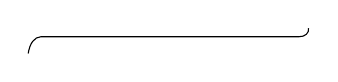
\begin{tikzpicture}[x=.4cm,y=.4cm,baseline=-.2ex]\draw (0,-.35) .. controls (.05,-.02) and (.2,.17) .. (.4,.18)--(8.6,.18) .. controls (8.80,.18) and (8.92,.3) .. (8.90,.45);\end{tikzpicture}}} The fact that one maps into $\mathrm{Projf}(k')$ \deleted{is expressed} and that the functor $G$ under consideration is exact is then expressed by the fact that the $L_{\handwritten{\alpha}}$ are \deleted{free}\inserted{projective} of finite type \uline{over} $k'$, and that the $L_{\handwritten{\unsure{\alpha|\mu}}}$ are f\rlap{r}l\rlap{e}at o\uline{ver the} $U_{\handwritten{\alpha}}$ (necessity trivial, sufficiency a little argument by reduction to the case $X$ simple, then $U$ a field equal to $X$ \ldots). Thus one finds exactly the \uline{modules} $L=(L_{\handwritten{\alpha}})$ \uline{over} $U'$ \uline{such that the} $\handwritten{L_\alpha}$ \uline{are flat over} $U_{\handwritten{\alpha}}$ \uline{and projective of finite type over} $k'$.
\margin{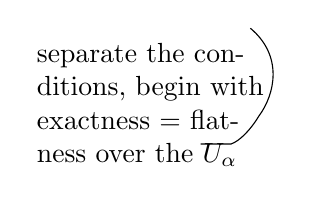
\begin{tikzpicture}[x=.35cm,y=.35cm,baseline=(n.base)]\node[anchor=north west,align=left,text width=3cm] (n) at (0,0) {separate the conditions, begin with exactness = flatness \handwritten{over the $U_\alpha$}};\draw (8.1,.2) .. controls (9.3,-.8) and (9.0,-2.2) .. (8.4,-3.0) .. controls (8.1,-3.5) and (7.7,-3.9) .. (7.4,-4.0)--(6.3,-4.0);\end{tikzpicture}}
$\mathbb{O}$n $\mathbb{t}\mathbb{h}\mathbb{e}$ other hand, independently of these \deleted{C}\inserted{\handwritten{\unsure{c}}\handwritten{\begin{tikzpicture}[x=.4cm,y=.4cm,baseline=-.2ex]\draw (0,.23)--(.14,0)--(.3,.21);\end{tikzpicture}}}onditions of flatness,\inserted{\handwritten{if in $C$ there are $1$ and $\vee$ compatible with\inserted{(\unsure{contravariance|contravariants})}\handwritten{\begin{tikzpicture}[x=.4cm,y=.4cm,baseline=-.2ex]\draw (0,-.35) .. controls (.05,-.02) and (.2,.17) .. (.4,.18)--(3.1,.18) .. controls (3.30,.18) and (3.42,.3) .. (3.40,.45);\end{tikzpicture}} $F$, i.e. $\Delta_U$ unital and $U$ with antipode}} the datum of an isomorphism $c$ amounts to the datum of an isomorphism of \inserted{\handwritten{right (*)}} bi-$U'$-modules
\margin{\deleted{\handwritten{\unsure{by dualizing it} \unsure{bringing in} \illegible{2} of an \unsure{antipode} $\unsure{U'}$}}}
\[
L\overset{\handwritten{\scriptscriptstyle\wedge}}{\otimes}_{\handwritten{k'}}L\handwritten{\xleftarrow{\sim}}L\overset{\handwritten{\scriptscriptstyle\wedge}}{\otimes}_{\handwritten{k'}}U'
\quad(\handwritten{\unsure{\simeq|\xrightarrow{\sim}}}L\otimes_{(U,\handwritten{\Delta})}(U\overset{\handwritten{\scriptscriptstyle\wedge}}{\otimes}_kU)\deleted{\handwritten{\unsure{\simeq}}}\handwritten{\simeq}L\otimes_{(U',\handwritten{\Delta'})}(U'\overset{\handwritten{\scriptscriptstyle\wedge}}{\otimes}_kU')).
\]
\inserted{\handwritten{[thanks to the antipode:) $x\otimes\unsure{U|u}\longrightarrow x\otimes(u\otimes1)$]}\handwritten{\begin{tikzpicture}[x=.4cm,y=.4cm,baseline=-.2ex]\draw (0,-.35) .. controls (.05,-.02) and (.2,.17) .. (.4,.18)--(3.2,.18) .. controls (3.40,.18) and (3.52,.3) .. (3.50,.45);\end{tikzpicture}}}

% source lines 24--26 and lower-margin notes
\deleted{In terms} Using the flatness conditions, one can define $B=\mathrm{Homcont}_{k'}(L,k')$, which is the inductive limit of the $B_{\handwritten{\alpha}}$ projective of finite type over $k'$ (a fortiori\inserted{\handwritten{it is}\handwritten{\begin{tikzpicture}[x=.4cm,y=.4cm,baseline=-.2ex]\draw (0,-.35) .. controls (.05,-.02) and (.2,.17) .. (.4,.18)--(1.4,.18) .. controls (1.60,.18) and (1.72,.3) .. (1.70,.45);\end{tikzpicture}}} flat over $k'$), and a coa\deleted{g}l\`{g}ebra over $A'$ (limit of coalgebras
\margin{\begin{tikzpicture}[x=.35cm,y=.35cm,baseline=(n.base)]\node[anchor=north west,align=left,text width=3.4cm] (n) at (0,0) {\handwritten{Let us begin \unsure{$U\to$|by} expressing everything on the side of $U,L$, and \handwritten{\begin{tikzpicture}[x=.4cm,y=.4cm,baseline=-.2ex]\draw[line width=.3pt] (.08,.28)--(.07,.02) .. controls (.15,-.11) and (.3,.02) .. (.35,.2)--(.43,-.06);\draw[line width=.55pt] (0,-.14)--(.32,.19);\fill[gray] (.08,.4) circle (.025);\end{tikzpicture}} dualize only at the end}};\draw (7.2,.8) .. controls (9.2,.7) and (8.8,-1.6) .. (9.7,-2.7) .. controls (10.2,-4.3) and (9.5,-5.8) .. (8.6,-6.8);\draw[line width=.2pt] (10.2,3.5) .. controls (10.1,1.0) and (10.6,-3.0) .. (10.4,-7.2);\end{tikzpicture}}
\handwritten{(*) The bimodule law in $L\otimes_{\unsure{U'|k'}}U'$ is given by}
\[
\handwritten{\left\{\begin{aligned}
&\text{first law : on the right by the }\unsure{\text{multiplications}}\text{ of }U'\\
&\text{second law : given by that of module : right}\\
&\text{over }U\otimes U^o\quad[U^o\text{ acts on the right on }U'\text{ !}]\\
&\text{via }(\mathrm{id}_U\otimes\underline{a}.)(\Delta_U)
\end{aligned}\right.}
\]
